%\documentclass[10pt,twocolumn]{article} % For LaTeX2e
\documentclass[10pt]{article} % For LaTeX2e
\usepackage{fullpage}
%\usepackage{nips12submit_e,times}
\usepackage{graphicx}
\usepackage{alexdefs}
%\documentstyle[nips12submit_09,times,art10]{article} % For LaTeX 2.09


\title{Computational Linguistics I Final Report}


\author{
Arti Ramesh, Scott White and Alex Memory \\
Department of Computer Science\\
University of Maryland\\
College Park, MD 20742 \\
}

\newcommand{\fix}{\marginpar{FIX}}
\newcommand{\new}{\marginpar{NEW}}

%\nipsfinalcopy % Uncomment for camera-ready version

\begin{document}

\maketitle

\begin{abstract}
    Semantic role labeling (SRL) is a task in which semantic labels for predicates and predicate arguments are assigned to constituents within the syntactic parse of a sentence, and is an approach for extracting meaning from sentences.  However, past machine learning approaches to SRL were limited by the availability of annotated SRL training corpora, and models trained on one corpus performed poorly on new corpora.  Our goal for this work was to use weak supervision to improve performance on unlabeled corpora or corpora in new domains while avoiding the expense of developing new training sets.  We evaluate our approach using the PropBank SRL training set, the database Freebase and the SwiRL SRL software; we discuss issues we encountered and suggest ways to refine the approach going forward.
\end{abstract}

%\section{Overview}
%\label{sec:overview}
%Blah blah intro.


\section{The Problem}
\label{sec:problem}
Semantic role labeling (SRL) is a task in which semantic labels for predicates and predicate arguments are assigned to constituents within the syntactic parse of a sentence, and is an approach for extracting meaning from sentences.
Early research on semantic role labeling (SRL) was seen in~\cite{gildea_automatic_2002} and ~\cite{chen_use_2003}, and after significant manual effort to annotate corpora as training sets, such as PropBank~\cite{kingsbury_adding_2002} and Framenet~\cite{ruppenhofer_framenet_2006}, machine learning (ML) approaches became common and achieved accuracy close to 80\%~\cite{carreras_introduction_2005}.
However, portability of trained models to unlabeled corpora remained a problem; even portability within the same domain, e.g. newswire, was poor~\cite{pradhan_towards_2008}.
Thus applications and further research on ML approaches was significantly limited by the number and variety of available training corpora, which are expensive to produce.
A low-cost approach to create novel training instances in new corpora, or even corpora in new domains, could increase the applicability and research on ML approaches to SRL.



\section{Our Approach}
\label{sec:approach}
To avoid the expense of creating training corpora, we employ a weak-learning approach in which the predicates in an existing training corpus are aligned to relations in a large external database, and instances of the database relations guide the search for novel training examples within another new corpus. 
If a learner is then be trained over a combination of the original training corpus and the new training examples, we hope that the resulting model has improved accuracy over the new corpus, compared to a model trained on the original training corpus alone.

Previous efforts to automatically find novel SRL training examples exist~\cite{furstenau_semi-supervised_2012}, but have not leveraged an external structured data source.
Weak supervision for relation extraction has been done previously~\cite{mintz_distant_2009}, but to our knowledge it was not applied to SRL specifically.


\subsection{Corpus to Database Alignment}
\label{sec:alignment}
The first step in our approach is to choose an existing SRL training corpus and align it to a large external database; for these we chose PropBank (PB) and Freebase~\cite{bollacker_freebase:_2008} (FB) respectively.
PropBank is an annotation layer on top of the Wall Street Journal portion of Penn Treebank II~\cite{marcus_building_1993}; for this reason, we expected better alignment if we only aligned PB to the business domain of FB.
We extracted the schema and predicate instances from PB using the Natural Language Toolkit~\cite{bird_nltk:_2006} and we retrieved the schema and relation instances from the business domain of FB from data dumps available on the FB web site.
Furthermore, we limited our alignment only to the most common predicates from PB.  The following figures illustrate the frequencies of common PB predicates and FB relations.

\begin{figure*} [ht]
\begin{center}
\subfigure[Propbank Verbs]{\label{fig:subfig1}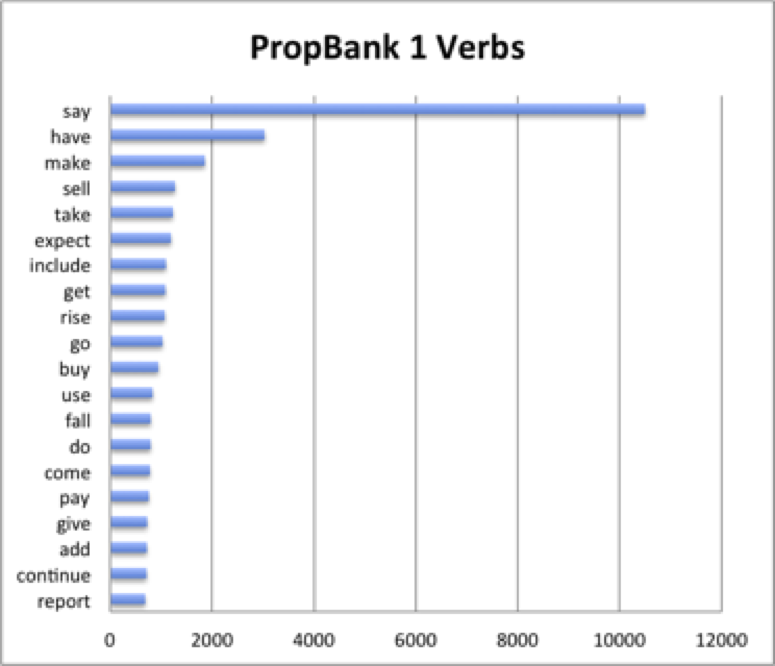
\includegraphics[width = 2.25in, height = 1.75in]{propverbs.png}}
\subfigure[Freebase Relations]{\label{fig:subfig2} 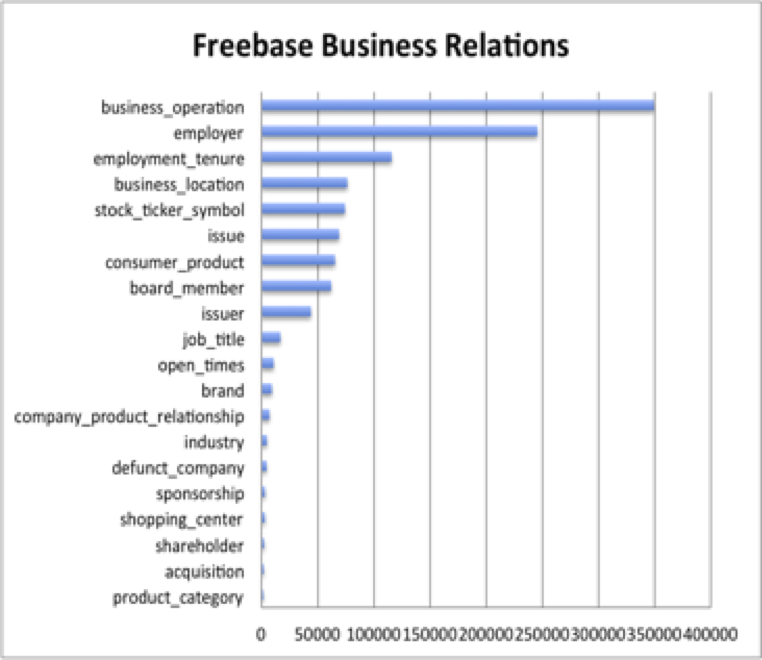
\includegraphics[width = 2.25in, height = 1.75in]{freebaserels.png}}
\caption{Frequency Distribution of Propbank Verbs and Freebase Relations}
\vspace{-0.5cm}
\label{fig:figure1}
\end{center}
\end{figure*}



The following table shows predicates and relations we expected to be aligned.

\begin{table} [ht]
\begin{center}
\small{
\begin{tabular}{p{3cm}p{4cm}p{4.5cm}}
\noalign{\smallskip}
\hline
Area & Propbank Verbs & Freebase Relations\\	
\hline
Advising & advise & company\_ advisor \\
Employment & employ, hire & employment\_ tenure, employer\\
Products & make, produce, market, sell & company\_product\_relationship\\
Purchasing	& acquire, purchase, sell	& acquisition\\
Sponsors	&sponsor	&sponsorship\\
Stock	&issue&	issue\\
\hline
\end{tabular}
}
\caption{Aligning Propbank verbs to Freebase relations}
\vspace{-0.4cm}
\end{center}
\end{table}

Our goal for alignment was to generate automatically mappings between the PB and FB at the schema level for relations and the arguments of the relations; for example the PB predicate acquire may map to the FB relation acquisition.
Furthermore, acquire has a roleset acquire.01 - in general, PB predicates may have multiple rolesets - which defines four numbered arguments including the agent acquiring something, the thing acquired and the price paid.
And, the FB relation acquisition has the arguments acquiring\_company and company\_acquired.
In this example, we want to align agent from PB to acquiring\_company from FB, etc. 

We performed the alignment using a probabilistic soft logic (PSL) program~\cite{brocheler_probabilistic_2012} comprising the data loaded from PB and FB, and logical rules which act as templates for a constrained continuous Markov random field.
The variables in the graphical model for a PSL program are real-valued, making it ideal for propagating similarity, such as string similarities, at the instance level between the two data sources to the schema level, which was our goal; and inferences are assigned truth values which allow us to set a minimum threshold to accept mappings.
We encoded the following three types of alignment rules in PSL.
(i) Using Levenshtein similarity to capture similarity between relation names, entity names and entity type names.
(ii) Transitivity:  if relation A is similar to relation B, and relation B to relation C, relation A and C are similar.
And (iii) Set similarity:  if the sets of instances of two relations are similar, then the relations are similar.
We now share two specific PSL rules that we used, and explanations of how they work.
\begin{align}
w_{1}: rel(I1,R1)\wedge rel(I2,R2) \wedge similar(R1,R2)&\rightarrow sameRel(R1,R2) \label{eq:rel_name}\\
w_{1}: rel(I1,R1)\wedge rel(I2,R2) \wedge similar(\left\{R1.entOf(inv)\right\},\left\{R2.entOf(inv)\right\}) &\rightarrow sameRel(R1, R2) \label{eq:ent_set}
\end{align}
% I made these rules simpler here so they would render nicely in latex.  -- Alex
In rule~\eqref{eq:rel_name} two relations R1 and R2 from PB and FB respectively are same relations if they are similar. Similarity is calculated using Levenshtein distance.
Rule~\eqref{eq:ent_set} is the set similarity feature in PSL used to compare two sets of values.
Here we compare the arguments of propbank to arguments of freebase and indicate a match if arguments are similar.
Instead of comparing each and every argument, a single rule in PSL can be used for comparing the sets.
Both rules have weight $w_1 = 20$.

The following table shows example output of our alignment on relations; upon inspection, it appears that mappings with higher truth values are quite close to what we expect.
Notably, the mapping between hire and employment was inferred through the transitive rule and similarity in argument instances, though the predicate and relation have dissimilar names.

\begin{table} [ht]
\begin{center}
\small{
\begin{tabular}{p{3cm}p{3cm}p{2cm}}
\noalign{\smallskip}
\hline
PB Predicate & FB Relation & Truth Value\\	
\hline
issue & issue & 1.0 \\
issue &issuer & 0.99  \\
issue & holding & 0.97\\
employ	& employment\_tenure	& 0.97\\
acquire	&acquisition	& 0.96\\
sponsor	&sponsorship&	 0.96\\
produce	&company\_product&	0.95\\
market	&employment\_tenure &	0.94\\
issue	&employment\_tenure &	0.94\\
sponsor & company\_advisor & 0.94\\
issue & company\_advisor & 0.94\\
advise & company\_advisor & 0.94\\
issue & asset\_ownership & 0.94\\
hire & employment\_tenure & 0.87\\

\hline
\end{tabular}
}
\caption{PSL Alignment Predictions}
\vspace{-0.4cm}
\end{center}
\end{table}





\subsection{Weak Supervision}
\label{sec:weak}
After finding correspondences between the PB and FB relations using PSL, we formed novel training instances of PB predicates from the corresponding FB relations.
To do this we, for each FB relation instance, found all the Treebank 2 (TB) sentences which contained the tokens from the instance FB arguments.
For efficiency, we limited our search to proper nouns within TB sentences.
Then, for each matching TB sentence, we chose the verb and argument locations for the PB annotation:  For the verb location, we chose the word which had the lowest edit distance from the baseform of the PB verb, and for the argument locations, we chose the locations of the longest token from each argument.
With the new PB annotation information thus chosen for each new instance, we added the new training instances to the original PB training set.

During the alignment step, we were unable to completely map the relation arguments between PB and FB, but after filling in argument spots in the mappings by hand, we began finding some novel training instances, although many of them were not direct instances of the PB predicates but did seem to match with a related sense or at a coarser level.
For example, for the {\tt acquire} predicate, we generated the new training sentence, “AEG is 80\% owned by Daimler-Benz AG, the country's biggest industrial concern.”
While this sentence does not include any form of the PB verb {\tt acquire}, it does match at the more abstract level of ownership that may be desirable when extracting meaning from sentences.

The final step was to train a SRL labeler on the expanded training set, and for this we used SwiRL~\cite{surdeanu_combination_2007}.
Before doing so, we needed to recombine the new PB layer with TB and convert the result into the correct input format for SwiRL.  Helpfully, the SRL shared task materials for CoNLL-2005 included all the necessary software to do this.



\section{Results and Challenges}
\label{sec:results}
Many steps in our approach proved to be challenging, required manual intervention to fully complete or produced a small quantity of output.  This was the case with alignment, where our results appeared promising but did not complete the mapping of arguments which we needed.  Consequently, we also had very few new instances for training SwiRL.  Ultimately, the accuracy result from training SwiRL on the expanded training corpus, seen in Table~\ref{tab:accuracy}, improved only slightly over the accuracy from training on the original PB corpus.
\begin{table}
\centering
\caption{SRL accuracy results with the original PropBank training corpus and with the novel instances found with our approach.}
\begin{tabular}{ | l | c | c | c |}
\hline
Training Set & Prec. & Rec. & F1 \\ \hline \hline
PropBank & 80.15 &  75.36 &  77.68 \\ \hline
PropBank + Novel Instances & 80.04 & 77.25 & 78.62 \\ \hline
\end{tabular}
\label{tab:accuracy}
\end{table}

In general, we encountered plenty of challenges handling the data and software involved, and in some cases have ideas for addressing or extending this work in the future.
\begin{itemize}
\item Because of lack of labeled data matching FB and PB entities, we could not learn the weights of the alignment rules in PSL. But if we can hand label data, then we can learn the weights on the rules.
\item Another challenge was that PropBank annotations, even within the same roleset, represent many word senses.
For example, for the issue.01 roleset, we have the sentence ``until Congress acts, the government hasn't any authority to issue new debt obligations of any kind, the Treasury said'' and ``SHAREDATA Inc. said it will amend a registration statement filed with the Securities and Exchange Commission to delete a plan to sell 500,000 newly issued common shares.''
Upon inspection, we see that the issue relation in Freebase corresponds to the latter sense but not the former.
This creates a challenge for our approach, especially our alignment phase in PSL, since one of our assumptions is that there is a single correspondence between a PB relation and a FB relation.
It may be that aligning PB rolesets to FB relations is not the right task; a better task may be to discover individual word senses within PB rolesets and align those to FB relations.
\item FB relations are sometimes specified in the form of Ids and instead of argument names and the argument names are specified in a separate file. That data was not used for our experiments due to lack of time. If we can extract the argument names corresponding to these relations as well using association mining, then we would have a larger dataset from Freebase as well.
\item We only explored the business domain from FB. There are other domains which can lead to a match between PB and FB and those can be used as well.
\item There were data formating issues in the corpuses which were larger than our expectation.  It was difficult to extract arguments from the corpus, and the extractions were very noisy for example ``Cray Computer which *T* -26,'' ``the perch and Dolphin fields,'' etc.
\item There were many missing values in the argument fields. Formatting the data for PSL to source turned out to be challenging as we had to fix the missing values and noisy extractions. The missing values created primary key violations when loaded into the PSL database.
\end{itemize}


\section{Conclusion}
\label{sec:conclusion}
Semantic role labeling is an approach for extracting meaning from sentences, but past machine learning approaches to SRL were limited by the availability of annotated SRL training corpora.  We developed an approach for weak supervision to improve performance on unlabeled corpora while avoiding the expense of developing new training sets.  We evaluated our approach and discussed the issues we encountered and future refinements that should follow from this work.



\bibliographystyle{plain} 
\bibliography{zotero}

\end{document}
